\section{Background} \label{Background}
\subsection{IMS Overview}

%\begin{comment}
\begin{figure}[!h]
        \centering
        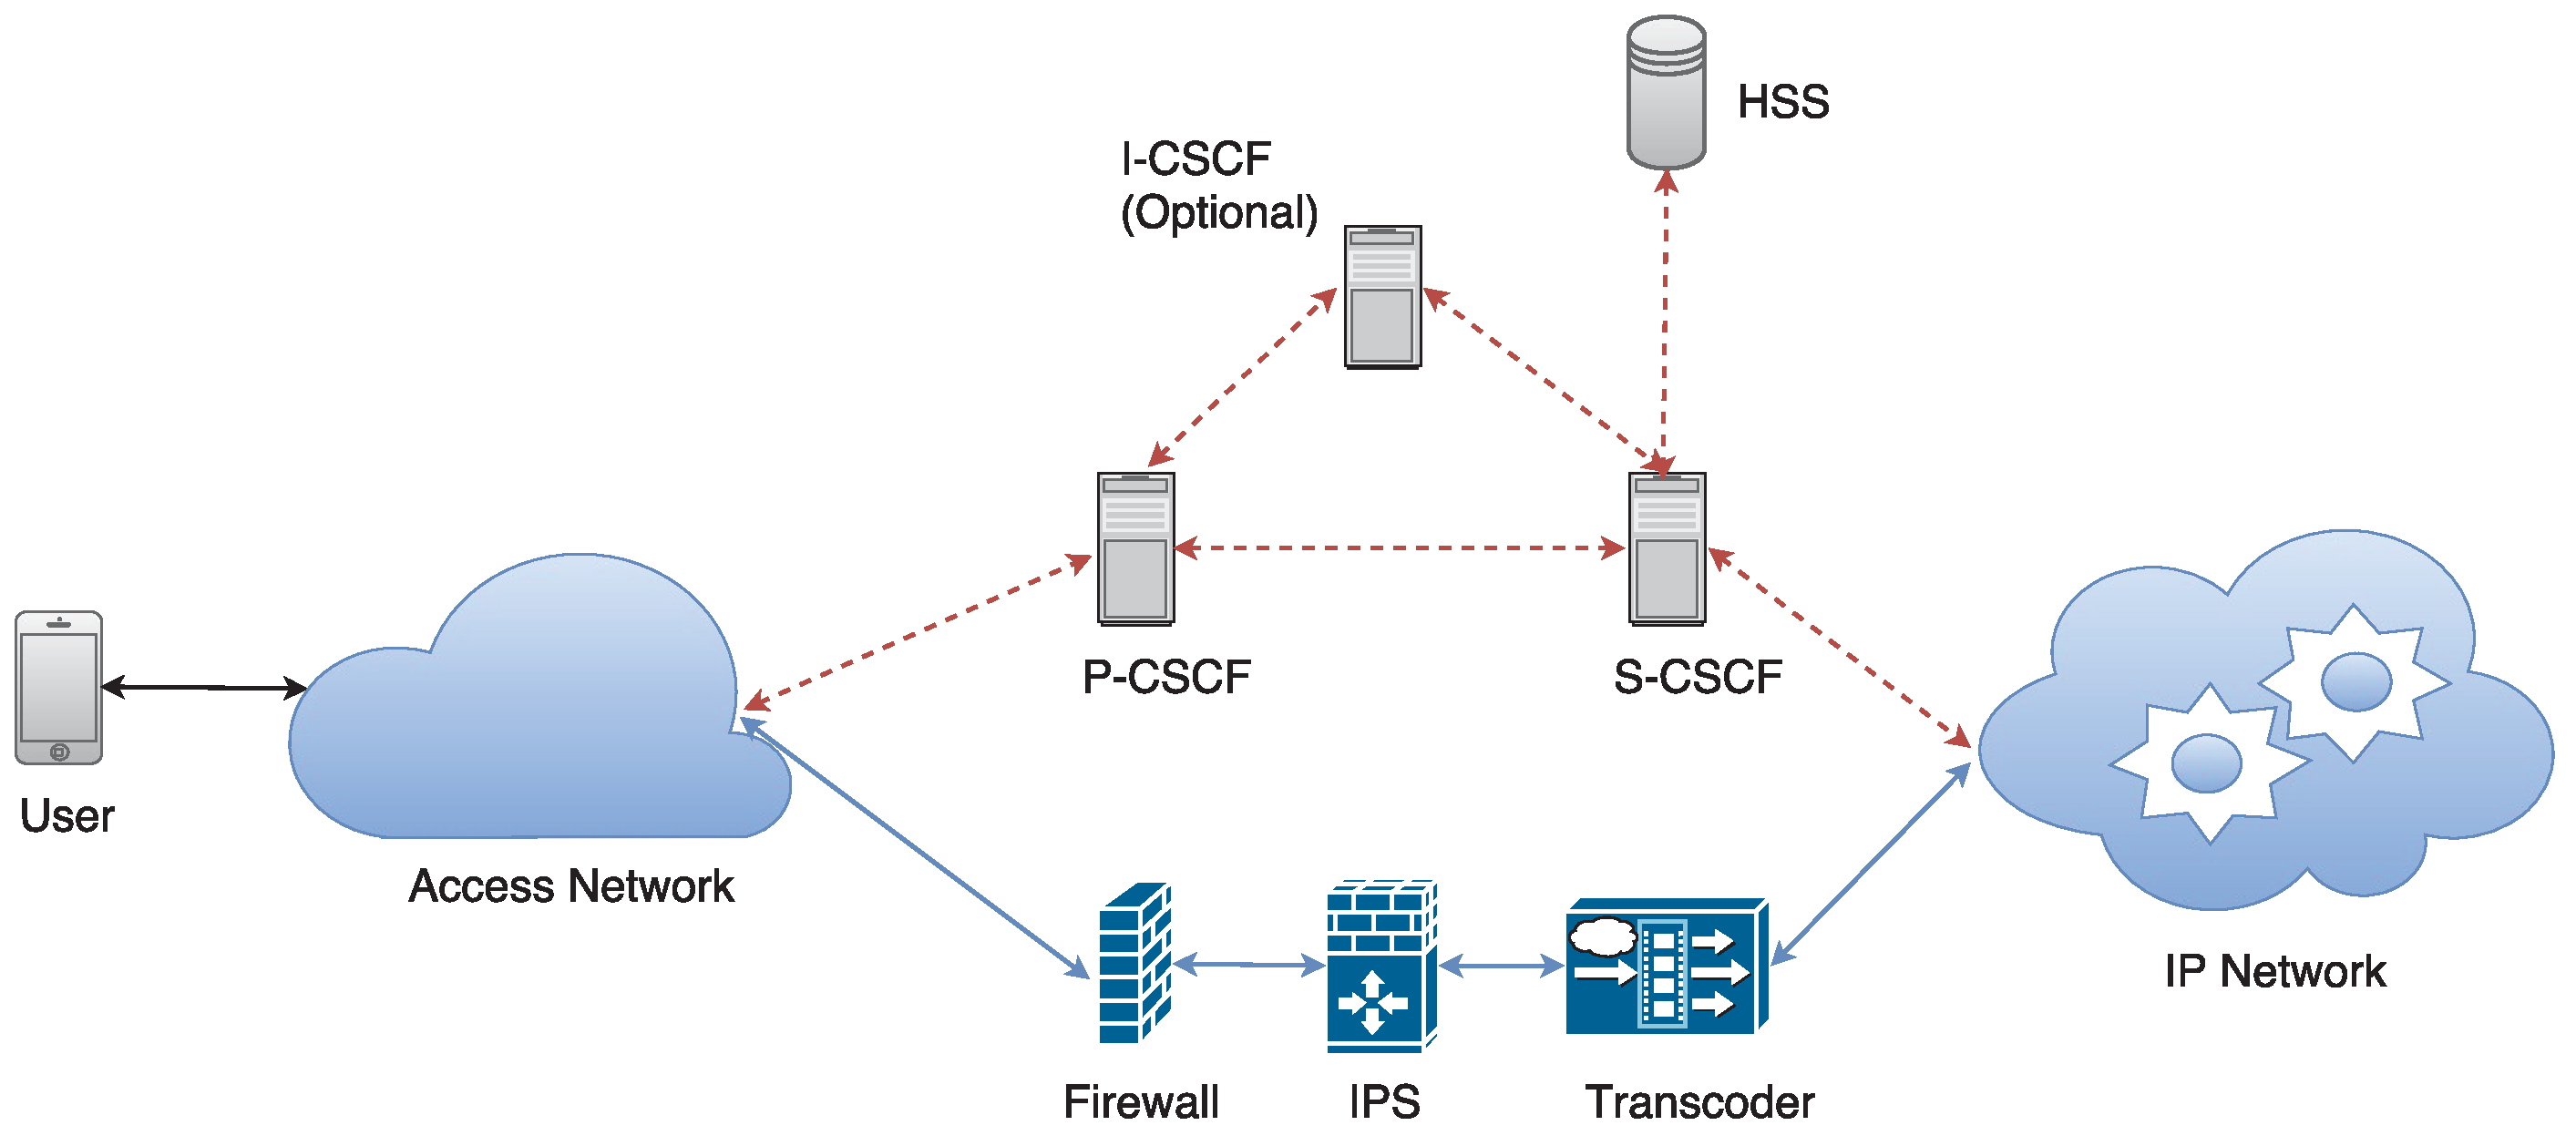
\includegraphics[width=1\columnwidth]{chap-scalims/figure/IMS_architecture.eps}
        \caption{IMS: an architectural overview}
        \label{fig:IMS_architecture}
\end{figure}
%\end{comment}

%cut for space
%old
%An IP Multimedia System (IMS) is a core part in 3G/4G telecom networks (e.g., 3GPP, 3GPP2)~\cite{umts}~\cite{lte}, responsible for delivering multimedia services (e.g., voice, video, messaging) over IP networks. IMS is a fully standardized solution for multimedia service delivery in the telecom industry~\cite{3gpp-ims}, as compared to its proprietary alternatives (e.g., Skype, Facetime). It is a complex system consisting of multiple service chains. We investigate two most important service chains as follows. An illustration is given in Fig.~\ref{fig:IMS_architecture}.
%new
An IP Multimedia Subsystem (IMS)~\cite{3gpp-ims} is a core part in 3G/4G telecom networks (e.g., 3GPP, 3GPP2)~\cite{umts}~\cite{lte}, responsible for delivering multimedia services (e.g., voice, video, messaging) over IP networks. It is a complex system consisting of multiple service chains. We investigate two most important service chains as follows. An illustration is given in Fig.~\ref{fig:IMS_architecture}.

$\triangleright$ \noindent\textbf{Control Plane (CP) Service Chain} includes three main network functions, {Proxy-CSCF (P-CSCF)}, {Interrogating-CSCF (I-CSCF)}, and {Serving-CSCF (S-CSCF)}, %collectively called Call Session Control Function (CSCF),
 which collectively handle user registration, user authentication and call setup. These network functions rely on the Session Initiation Protocol (SIP)~\cite{sip} to interoperate with users of the IMS system. Users can only contact with P-CSCF, which acts as a relay point between users and S-CSCF. Since I-CSCF acts as a middleman that forwards SIP messages between P-CSCF and S-CSCF, real-world implementation sometimes merges I-CSCF into S-CSCF as in \cite{project-clearwater} to simplify the structure of the IMS control plane service chain, making I-CSCF optional. S-CSCF %is the pivot on the control plane. It
  dispatches SIP messages to their final destinations and constantly queries an external storage server called Home Subscriber Server (HSS), which is a database that contains identities of the users. We consider the control plane service chain $\text{P-CSCF} \rightarrow \text{S-CSCF} \rightarrow \text{P-CSCF}$ in \textit{ScalIMS}. % scales the simplified control plane service chain, which has the form of $\text{P-CSCF} \rightarrow \text{S-CSCF} \rightarrow \text{P-CSCF}$.


\begin{comment}
\vspace{-3mm}
\begin{table}[!h]
        \small
        \begin{center}
        \begin{tabular}{p{0.15\linewidth}|p{0.7\linewidth}}
                %\hline
                %NF  & Description\\
                \hline
                P-CSCF & Point of attachment of a user to the IMS. Assigned to user and remains unchanged all time.\\
                \hline
                I-CSCF & Optional for security reason, forwards SIP request or response to the S-CSCF.\\
                \hline
                S-CSCF & Handles SIP message with the help of HSS, and binds the user IP address and the SIP address.\\
                \hline
        \end{tabular}
       % \caption{Network functions for the IMS control plane}
       % \label{tab:control-plane}

        \end{center}
\end{table}
\end{comment}

$\triangleright$ \noindent\textbf{Data Plane (DP) Service Chain} contains a sequence of network functions that the actual multimedia traffic between users traverses, for security (e.g., firewall, deep packet inspection, intrusion detection), connectivity (e.g., NAT, IPv4-to-IPv6 conversion), quality of service (e.g., traffic shaping, rate limiting, ToS/DSCP bit setting), and media processing (e.g., transcoding). While 3GPP has standardized the IMS control plane for interoperability reasons, the exact set of deployed network functions for the data plane varies per operator.


The two service chains collectively handle two important procedures of the IMS system, which are user registration and call setup. %User registration is performed through a SIP REGISTRATION transaction over the control plane.
To make a call, a user first registers his IP address to the IMS by initiating a SIP REGISTRATION transaction over the CP. When the registration is done, S-CSCF temporarily stores the binding between the identity of the user and the P-CSCF instance connected to the user for future calls. To setup a call between a caller and a callee, the caller initiates a SIP INVITE transaction to the IMS, specifying the identify of the callee. S-CSCF uses the binding saved during user registration to retrieve the P-CSCF instance that the callee connects to and sends the message to the P-CSCF instance, which forwards to the callee. After the callee responds, a call is successfully set up. Subsequent media flows between the caller and the callee are routed through DP service chain. When the call is finished, a SIP BYE transaction between the caller and the callee is carried out to close the call over the CP.

%A good NFV management system should effectively scales both the control and data plane service chains of the IMS system. %Since the operation of these two service chains are coupled together through SIP protocol, \textit{ScalIMS} uses a novel method based on flow tagging to effectively scale these two service chains.

\subsection{Related Work}

%In recent years, researchers have pay great attention to NFV technology. By running VNF softwares in virtual machines on computing clusters~\cite{palkar2015e2} or on cloud~\cite{sherry2012making}~\cite{lan2016embark}, service providers could be freed from managing complicated hardware network functions and deploy service chains at ease.

%Performance and scalability of using VNFs in the place of hardware middleboxes have been the focuses of investigation in the existing literature on NFV.

%\noindent \textbf{Performance.}
Running VNF software (e.g., DP packet processing software) on VMs incurs significant context switching cost~\cite{rizzo2013speeding}, limiting the maximum throughput of a VNF. To solve this problem, ClickOS~\cite{martins2014clickos} maps packets directly from NIC receive queues to a shared memory region, and fetch packets directly from that shared memory region~\cite{dpdk}, which greatly improve packet processing throughput. However, this approach completely by-passes the existing kernel networking stack, unable to support VNFs (e.g., S-CSCF and P-CSCF used by IMS system) that use the traditional TCP/IP stack. %
%lose flexibility for network programability (i.e. SDN~\cite{mckeown2008openflow} functionality provided by OpenvSwitch~\cite{pfaff2015design}). On the other hand, some control-plane VNFs (e.g., P-CSCF and S-CSCF as in the Clearwater Project~\cite{project-clearwater}) function well enough on existing network stacks as they are application-level software. If enough scalability is given, existing network stacks could still be used to build NFV service chains.

%\noindent \textbf{Scalability.}
Scaling of service chains has been investigated in a single server, a computing cluster or a datacenter. CoMB~\cite{sekar2012design} focus on scaling VNFs in a single server, %for better performance. %Even though their implementations achieve good performance, but it lacks generality and flexibility.
 by designing customized architecture to unify VNFs inside a single server. % and they can not be cannot be seemlessly integrated into existing SDN framework.
 %E2~\cite{palkar2015e2}, Stratos~\cite{gember2012stratos} and Slick~\cite{anwer2015programming} study scaling of VNFs in a single SDN-enabled datacenter.
 E2~\cite{palkar2015e2} scales VNF service chains in a single datacenter, %scales VNF instances  within a computing cluster connected through SDN enabled switches through
 exploiting high-performance inter-VNF data paths through SDN-enabled switches. % it has its own high performance inter-VNF datapath.
Stratos~\cite{gember2012stratos} %scales VNF instances by
 jointly consider VNF placement and flow distribution within a datacenter, using on-demand VNF provisioning and VM migration to mitigate hotspots.

%To our knowledge, there do not exist NFV management frameworks that scale VNF service chains across geo-distributed datacenters. % while \textit{ScalIMS} concentrates on scaling NFV service chains across datacenters.
The management systems mentioned above cannot be directly extended to the multi-datacenter setting. One primary reason is that SDN controllers~\cite{mckeown2008openflow} are extensively used in these systems to facilitate routing, scaling and load-balancing within a datacenter. However, SDN controllers are rarely available in the WAN, except for among datacenters of a few large providers such as Google~\cite{jain2013b4} and Microsoft~\cite{hong2013achieving}.
%\chuan{change this reference to B4 or SWAN}. %It is extremely hard for a SDN controller to set up flows on other datacenters, which incurs too much delay and hurts flow performance. One possible approach is to deploy one SDN-enabled management system in each datacenter, but there is no existing work on coordinating the behavior of such independent scaling systems, needed for deploying and scaling geo-distributed service chains. %However, scaling systems on different datacenters need to agree on complicated task such as coordinated VNF instance provision and collective flow routing. And all these problems call for an efficient design of a multi-datacenter scaling system.
%A new management system is in need, that efficiently coordinates service chain deployment and scaling, as well as flow routing, across multiple data centers.
 \textit{ScalIMS} is a NFV management system that efficiently coordinates service chain deployment and scaling, as well as flow routing, across multiple data centers. \textit{ScalIMS} uses similar methodologies as in~\cite{palkar2015e2} and \cite{gember2012stratos} when scaling NFV service chains within a datacenter, but adopts a novel distributed flow routing approach and a proactive scaling strategy to scale NFV service chains across multiple datacenters.

Similar with \textit{ScalIMS}, Klein \cite{qazi2016klein} also scales NFV service chains across multiple datacenters. However, it focuses on scaling EPC system \cite{epc} and does not use a hybrid scaling strategy as \textit{ScalIMS} does. Ren et al. \cite{ren2016dynamic} propose a VNF dynamic auto scaling algorithm for 5G networks, but it lacks a real-world implementation when compared to \textit{ScalIMS}.
